\subsection{Periodicity Tasks}\label{synth-benchmark:periodicity}


We introduce a family of synthetic tasks designed to evaluate temporal graph learning (TGL) methods' ability to recognize periodic structures. These tasks assess two fundamental capabilities: \emph{counting} and \emph{memorization}, in both deterministic and stochastic environments.


\begin{figure}[ht]
    \centering
    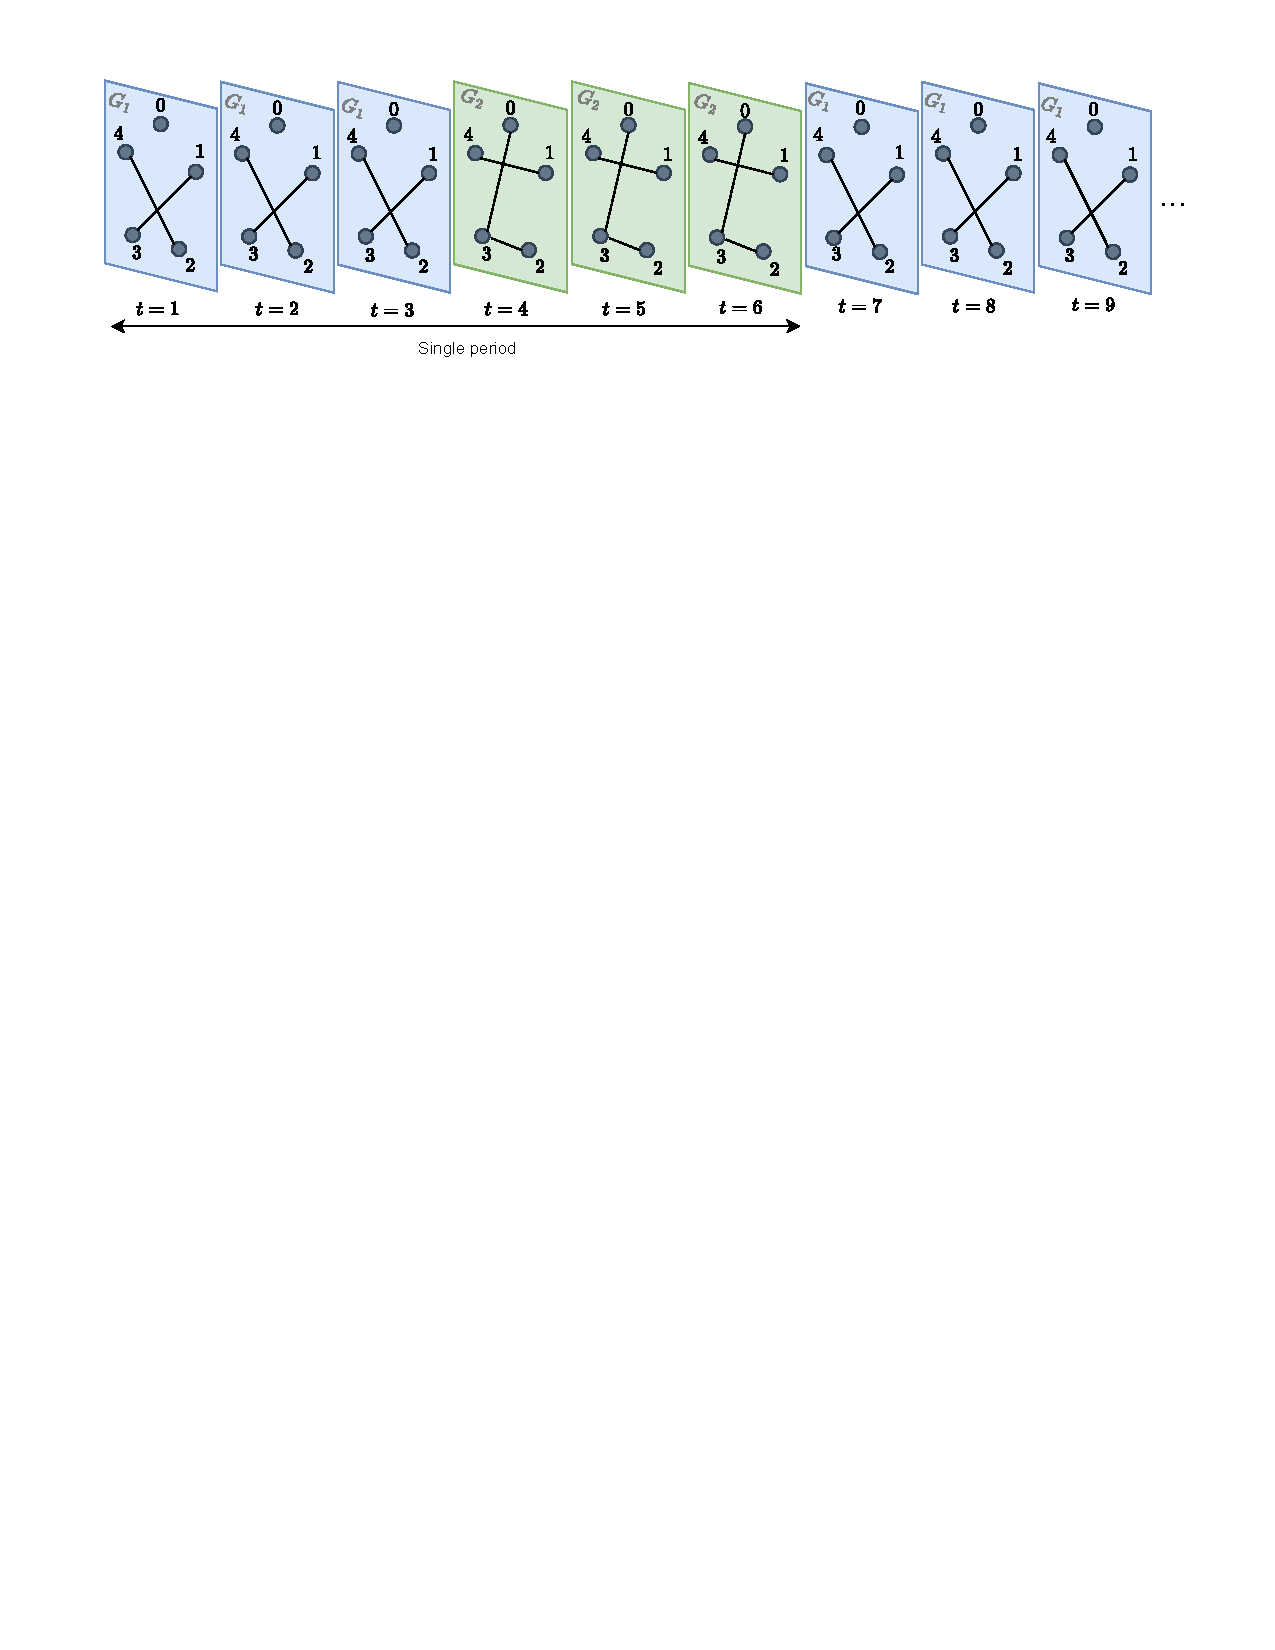
\includegraphics[width=\linewidth, height=8em, keepaspectratio]{figs/periodicity/Fixed_ER/(2, 3)_dataset.pdf}
    \caption{Periodic task in $\Pdet{k\!=\!2,n\!=\!3}$ with 2 unique snapshots repeated 3 times within a  period. }
    \label{fig:periodicity}
\end{figure}


\begin{definition}[Periodicity Tasks]
Let $k, n \in \mathbb{N}$. The task families $\Pdet{k,n}$ and $\Psto{k,n}$ are defined based on a repeating pattern where integers $i=1,\dots,k$ each appears $n$ consecutive times before cycling. For each $t$, let $i_t = (\lfloor t/n\rfloor \mod k) + 1$.
In $\Pdet{k,n}$, the dynamic graph $\mathcal{G} = G_1, G_2, \dots$ is a periodic sequence alternating between $k$ fixed static graphs $G_1, \dots, G_k$, i.e., $G_t = G_{i_t}$.
In $\Psto{k,n}$, each $G_t$ is sampled from one of $k$ distributions $D_1, \dots, D_k$ over static graphs (e.g., Erd\H{o}s-Rényi~(ER)~\cite{erdos1960evolution}, Stochastic Block Model~(SBM)~\cite{holland1983stochastic}), with $G_t \sim D_{i_t}$. The resulting sequence is stochastic, but the distribution pattern follows the periodic structure of $\Pdet{k,n}$.
\end{definition}

For example, a task in $\Pdet{k\!=\!3,n\!=\!2}$  will correspond to a dynamic graph $ G_1,G_1,G_2,G_2,$ $G_3,G_3,G_1,G_1,$..., where $G_1,G_2,G_3$ are static graphs. A task in $\Pdet{k,n}$ is illustrated in Figure~\ref{fig:periodicity}.


\textbf{Task objectives.}
Tasks in $\Pdet{k,n}$ test the counting and memory capacity of TGL methods. The parameter $k$ controls the length of the pattern and thus the memory demand, while $n$ governs how long each graph is repeated and tests the model's ability to count. For instance, solving a task in $\Pdet{2,n}$ requires counting up to $n$ before switching graphs, while solving a task in $\Pdet{k,1}$ requires memorizing $k$ static graphs. Tasks in $\Psto{k,n}$ introduce stochasticity, requiring models to reason over distributions rather than fixed structures, increasing the complexity while retaining the same periodic structure.
%Detailed dataset statistics for these tasks can be found in \Cref{appendix:periodicity-deterministic-stats}.


\begin{figure*}
    \centering
    \begin{subfigure}[b]{0.3\textwidth}
        \centering
        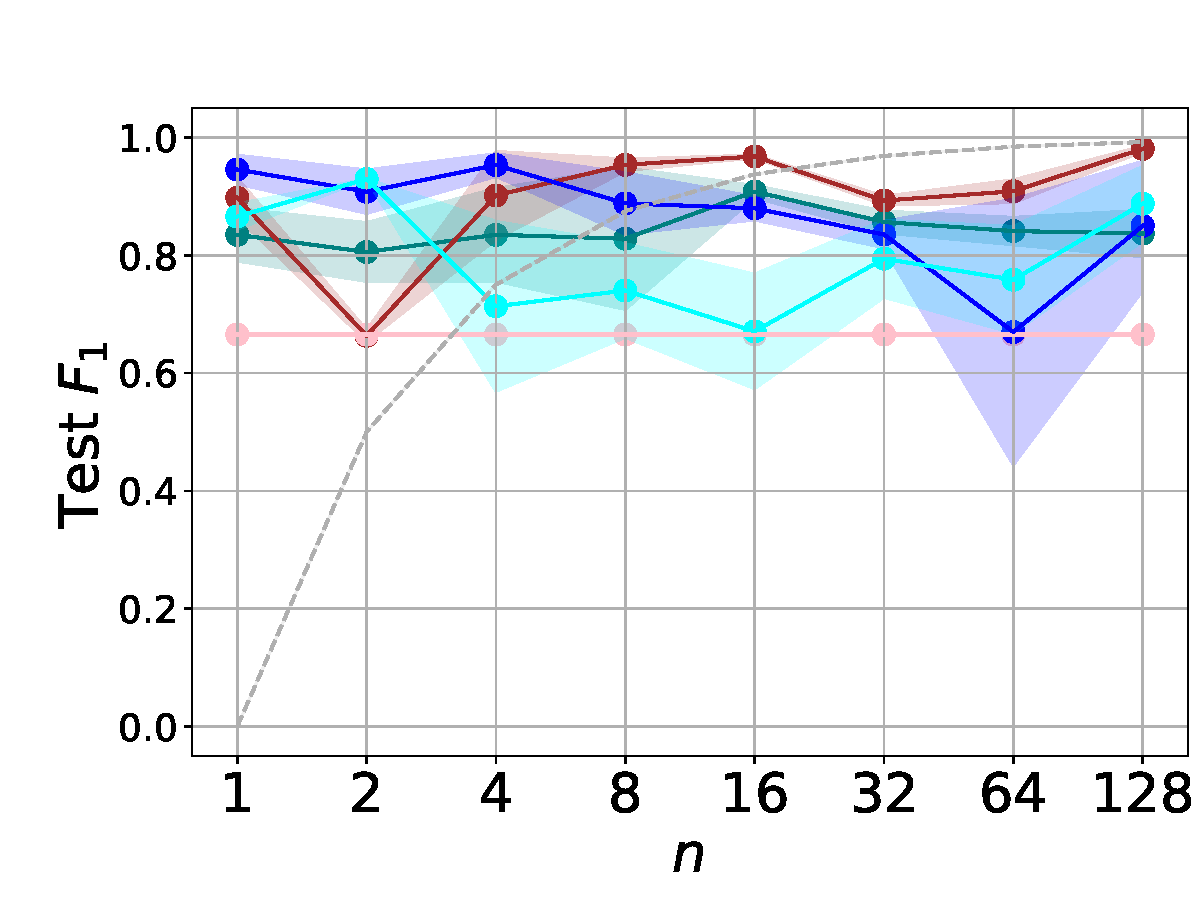
\includegraphics[width=\linewidth,trim={0 2.25cm 0 0},clip]{figs/periodicity/Fixed_ER/(2, n)CTDG_Test $F_1$.pdf}      
        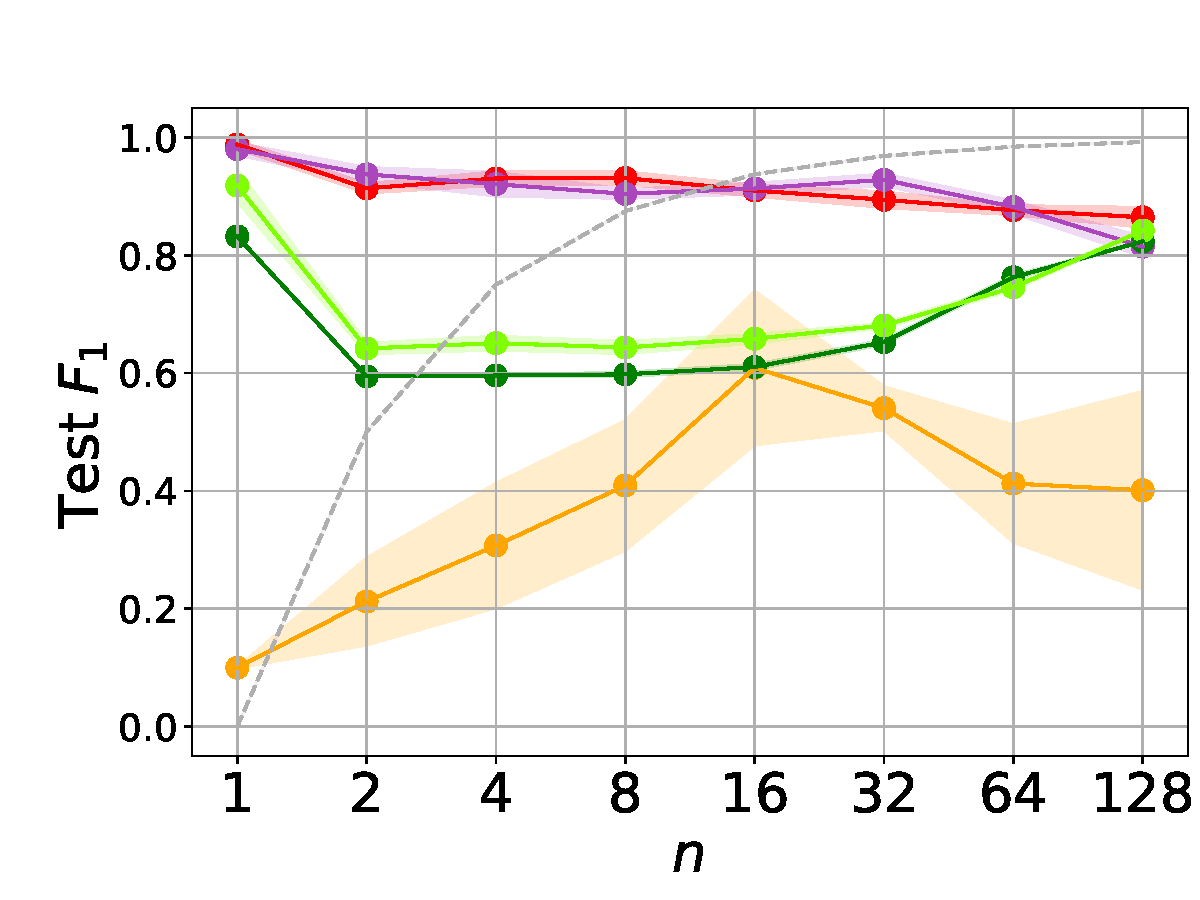
\includegraphics[width=\linewidth,trim={0 0 0 1.2cm },clip]{figs/periodicity/Fixed_ER/(2, n)DTDG_Test $F_1$.pdf}
        \caption{$\Pdet{2,n}$ - All time steps.}
        \label{fig:dtdg_(2,n)_allsteps}
    \end{subfigure}
    \begin{subfigure}[b]{0.3\textwidth}
        \centering
        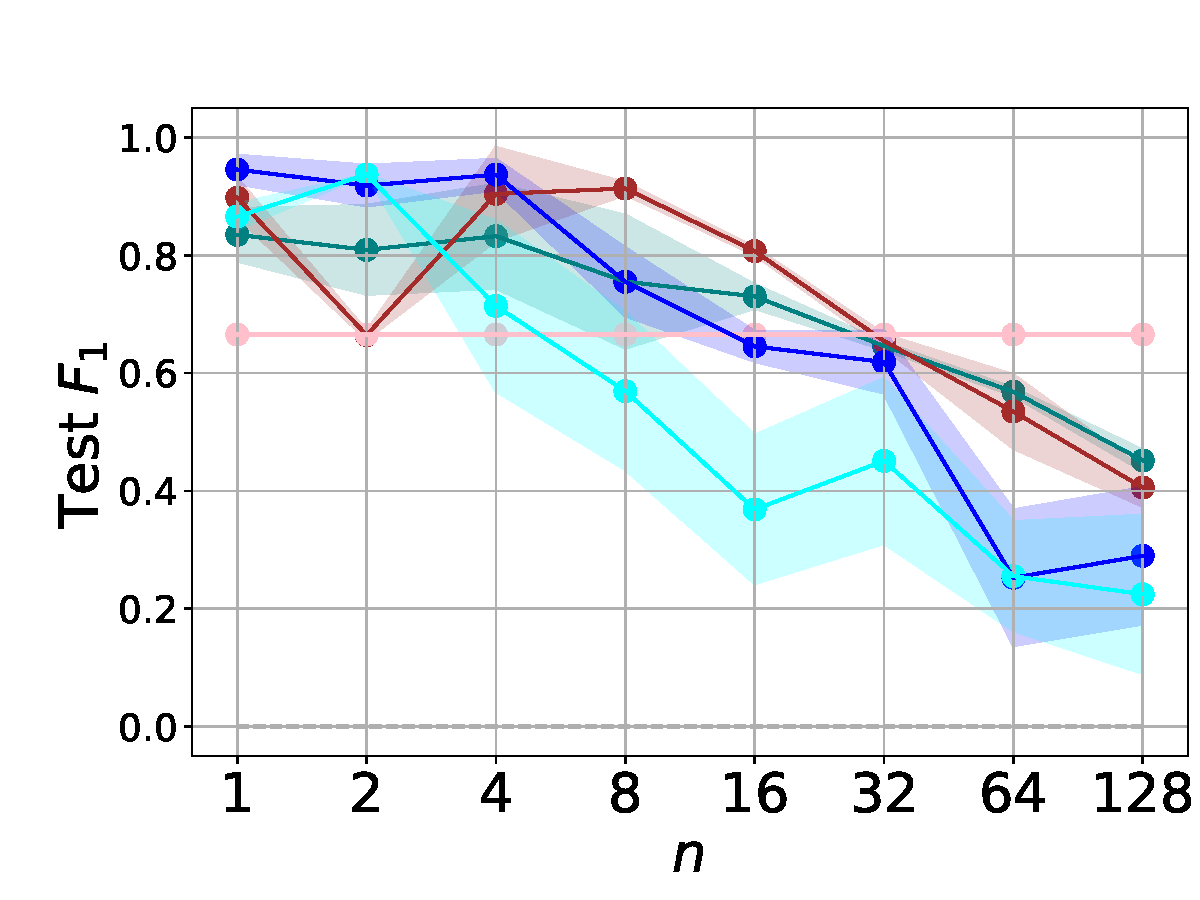
\includegraphics[width=\linewidth,trim={0 2.25cm 0 0},clip]{figs/periodicity/Fixed_ER/change_point/(2, n)CTDG_CP_Test $F_1$.pdf}
        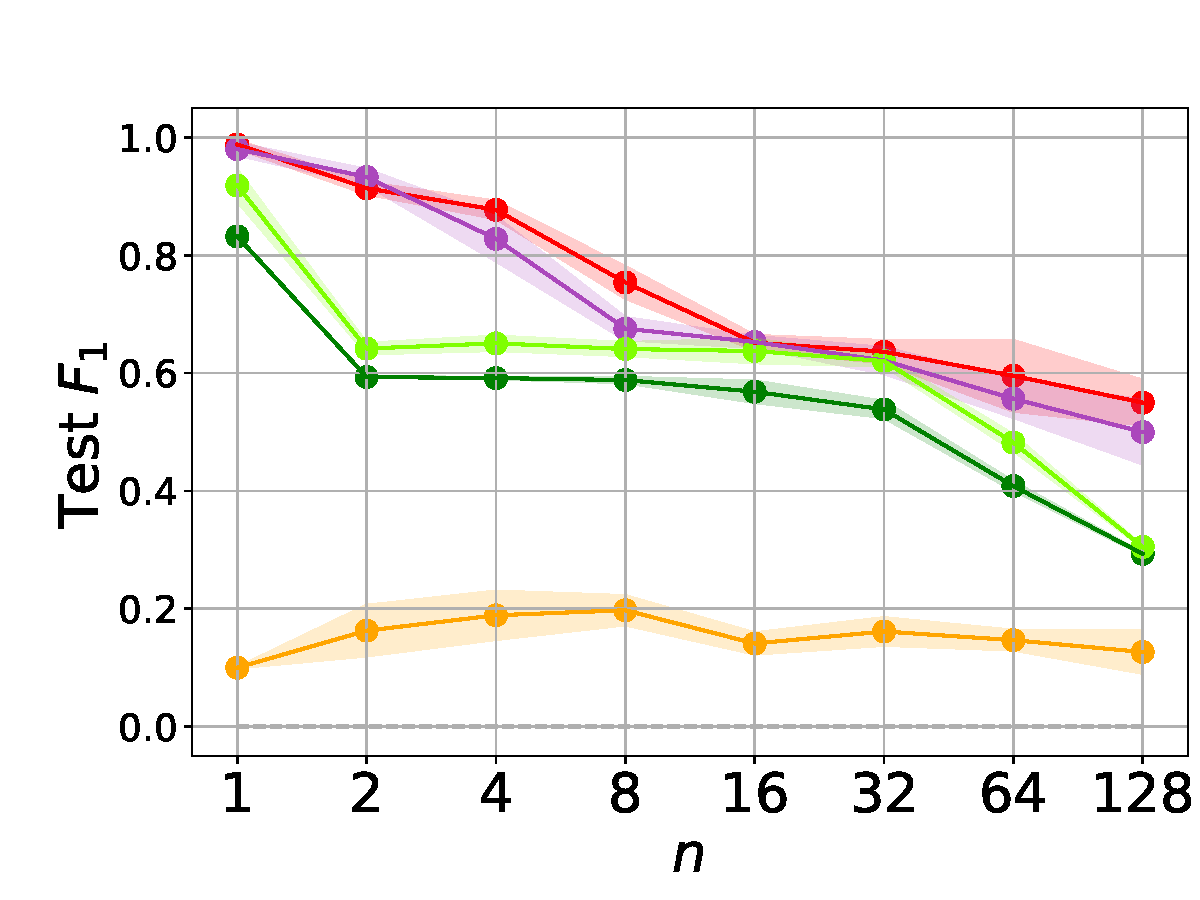
\includegraphics[width=\linewidth,trim={0 0 0 1.2cm },clip]{figs/periodicity/Fixed_ER/change_point/(2, n)DTDG_CP_Test $F_1$.pdf}
        \caption{ $\Pdet{2,n}$ - Change points.}
        \label{fig:dtdg_(2,n)_changepoints}
    \end{subfigure}
    \begin{subfigure}[b]{0.3\textwidth}
        \centering
        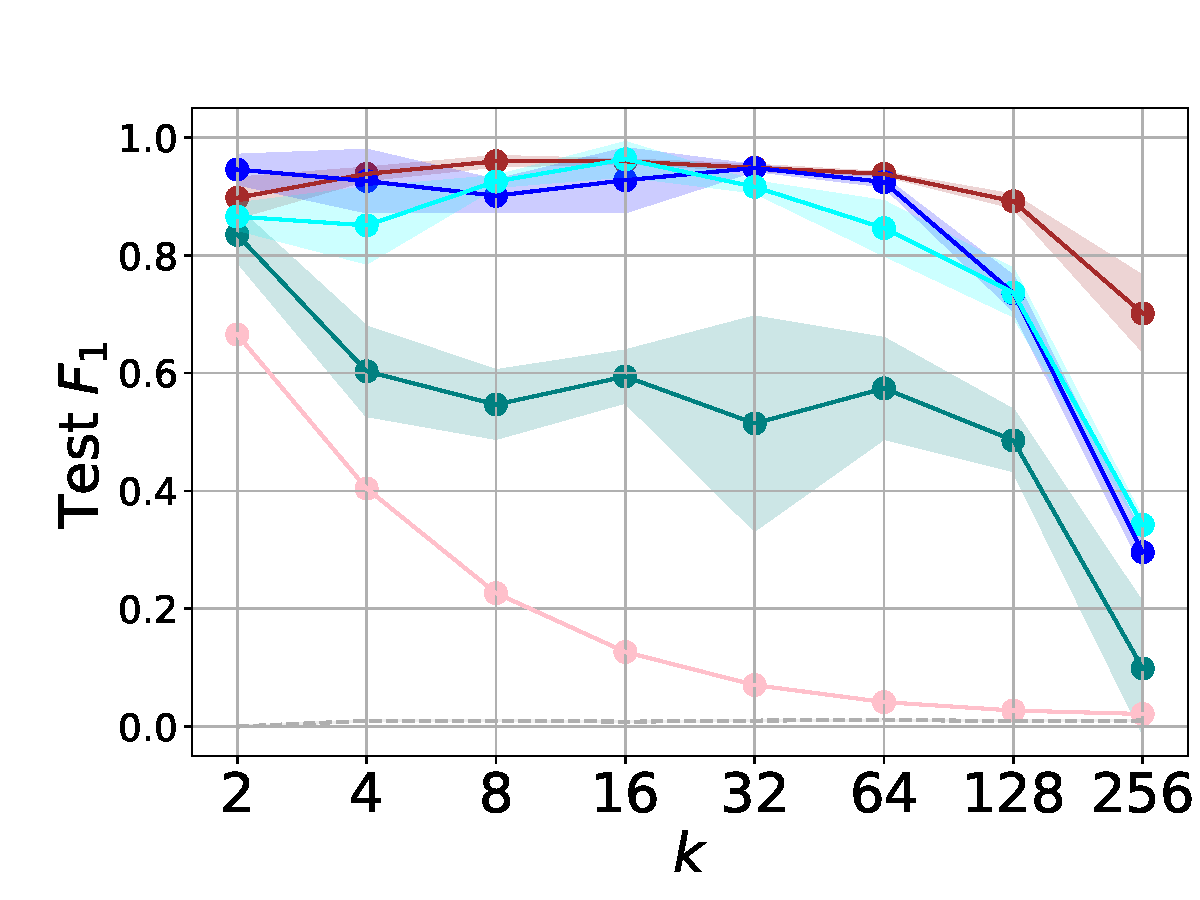
\includegraphics[width=\linewidth,trim={0 2.25cm 0 0},clip]{figs/periodicity/Fixed_ER/(k, 1)CTDG_Test $F_1$.pdf}
        
        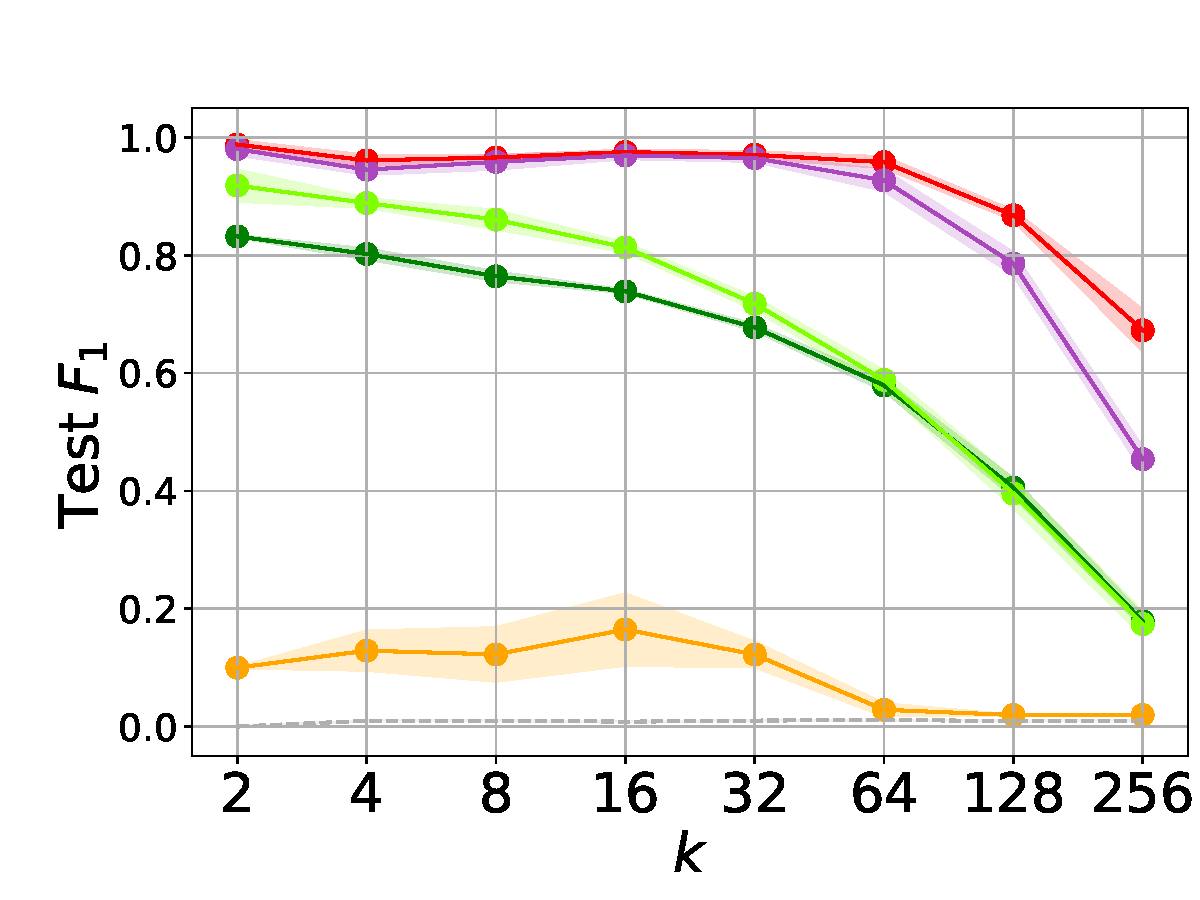
\includegraphics[width=\linewidth,trim={0 0 0 1.2cm },clip]{figs/periodicity/Fixed_ER/(k, 1)DTDG_Test $F_1$.pdf}
        \caption{$\Pdet{k, 1}$ - All time steps.}
        \label{fig:dtdg_(k, 1)}
    \end{subfigure}
    \begin{subfigure}[b]{0.08\textwidth}
        \centering
        \raisebox{14mm}{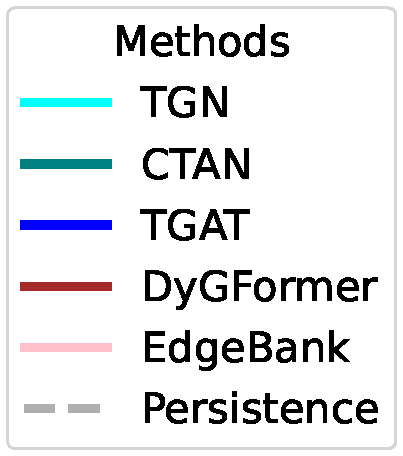
\includegraphics[width=\linewidth]{figs/legends/CTDG w persistence.pdf}}
        
        \raisebox{14mm}{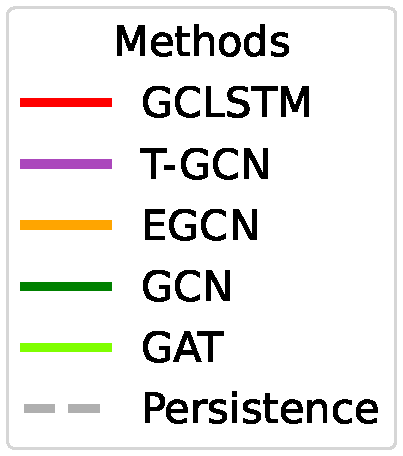
\includegraphics[width=\linewidth]{figs/legends/DTDG w persistence.pdf}}
    \end{subfigure}
    
    \caption{
    Performance of CTDG methods (top row) and DTDG methods (bottom row) on the deterministic periodicity tasks.
    %$\Pdet{2, n}$~(left and center) and $\Pdet{k, 1}$~(right). 
    }
    \label{fig:det_periodic_overall}
\end{figure*}

\looseness-1 \textbf{Can TGNNs count?} To evaluate the counting ability of TGNNs, we construct tasks in $\Pdet{k,n}$ with graphs sampled from the Erdős-Rényi (ER) model~\citep{erdos1960evolution} (100 nodes, edge probability 0.01). We set $k = 2$ and vary $n$, where increasing $n$ corresponds to greater task difficulty as models must count longer sequences.

Model performance on these $\Pdet{2,n}$ tasks for $n$ ranging from 1 to 128 is presented in \Cref{fig:det_periodic_overall}. 
Since models that simply repeat the previous timestep can perform well for large $n$, we evaluate both overall performance~(left plot) and performance at change points~(center plot) where the active graph switches (i.e., $t = n+1, 2n+1, \cdots$). High scores at change points indicate true counting and pattern understanding, whereas good overall performance with poor change point performance suggests the model is merely exploiting continuity rather than reasoning about periodicity.

%We report the $F_1$ score for dynamic link prediction in two ways: over all timesteps (left plot) and exclusively at change points (center plot).

\looseness-1 The results reveal distinct behaviors across different TGNN families. Among CTDG models, TGAT excels for small $n$, while DyGFormer demonstrates more consistent performance at larger $n$. For DTDG methods, T-GCN and GC-LSTM are strongest overall. Notably, EvolveGCN performs worse than static graph learning methods (GCN and GAT), which lack temporal processing mechanisms, underscoring how challenging these seemingly simple periodic patterns can be for current TGNNs. EdgeBank remains constant across all $n$ values, always predicting the union of both graphs. The persistence baseline improves over all timesteps as $n$ increases by simply copying the previous snapshot, but scores zero at change points.

\looseness-1 A key observation, evident when comparing performance over all timesteps versus at change points (\Cref{fig:det_periodic_overall}), is that as $n$ grows, many models increasingly rely on repetition rather than explicit counting. While their overall scores might remain high or even improve for larger $n$ (due to successfully predicting links during long static phases), their performance at change points often degrades. At $n = 32$, EdgeBank even starts to outperform all TGNNs. This divergence suggests that current TGNNs struggle to robustly count long sequences and instead learn a simpler heuristic reminiscent of persistence. %Further per-timestep analysis supporting this trend is provided in Appendix~\ref{appendix:pertimesteps_counting}.

\looseness-1 \textbf{How much can TGNNs memorize?} To evaluate the memorization capabilities of TGNNs, we fix $n = 1$ and vary $k$. The difficulty scales with $k$: as more unique graph structures are introduced, models must maintain a larger and more distinct set of representations to correctly predict links at each timestep. \label{seq:memorize}

\looseness-1 Figure~\ref{fig:det_periodic_overall} (right) shows results on $\Pdet{k, 1}$ for $k$ ranging from 2 to 256. As expected, EdgeBank steadily degrades to zero performance at $k = 256$, eventually defaulting to predicting each snapshot as a clique. All TGNN models show a gradual decline as $k$ increases. GC-LSTM and DyGFormer consistently perform best, demonstrating strong memorization of patterns. T-GCN, TGN, and TGAT remain robust up to $k = 128$, but drop sharply at $k = 256$, suggesting these models reach their maximum memorization capacity at this point.

\looseness-1 In contrast, TGNNs such as CTAN and EvolveGCN struggle significantly as the number of unique graphs increases. CTAN's performance begins to degrade considerably after $k=64$. Notably, both these methods are often outperformed by static GNNs like GCN and GAT, which exhibit a more gradual decline. This suggests that for tasks dominated by the need to memorize distinct states, an ineffective temporal mechanism can be more detrimental than no temporal mechanism at all.

\looseness-1 \textbf{Can TGNNs learn stochastic periodic structures?} Finally, we investigate how models' memorization capabilities extend to probabilistic settings, where periodic structure emerges from stochastic processes rather than deterministic patterns. 
We employ Stochastic Block Models (SBMs) with 100 nodes divided into 3 communities. While all SBM distributions share identical inter-community (0.01) edge probabilities, they differ in community structures 
%(details in Appendix~\ref{appendix:periodicity_stochastic_design})
. We examine two intra-community edge probability settings: $p=0.9$ and $p=0.5$~(the latter being  more difficult). 

Figure~\ref{fig:(K,1)_overall_sto} presents model performance across these stochastic periodicity tasks. As expected, performance decreases as $k$ increases, reflecting the growing challenge of memorizing multiple stochastic patterns. GC-LSTM consistently achieves the highest performance across both probability settings, with TGAT as the second-best performer. While T-GCN performs strongly with clearer community structure ($p=0.9$), it struggles in the noisier setting ($p=0.5$), falling behind TGAT and TGN. Overall, performance decreases under lower intra-community density, confirming that increased stochasticity challenges memorization capabilities. Notably, unlike in deterministic scenarios, static baselines (GCN and GAT) consistently underperform temporal models, highlighting the effectiveness of temporal modeling in capturing stochastic periodic structures within dynamic graphs.

\begin{figure}
    % (k, 1) CTDG
    \centering
        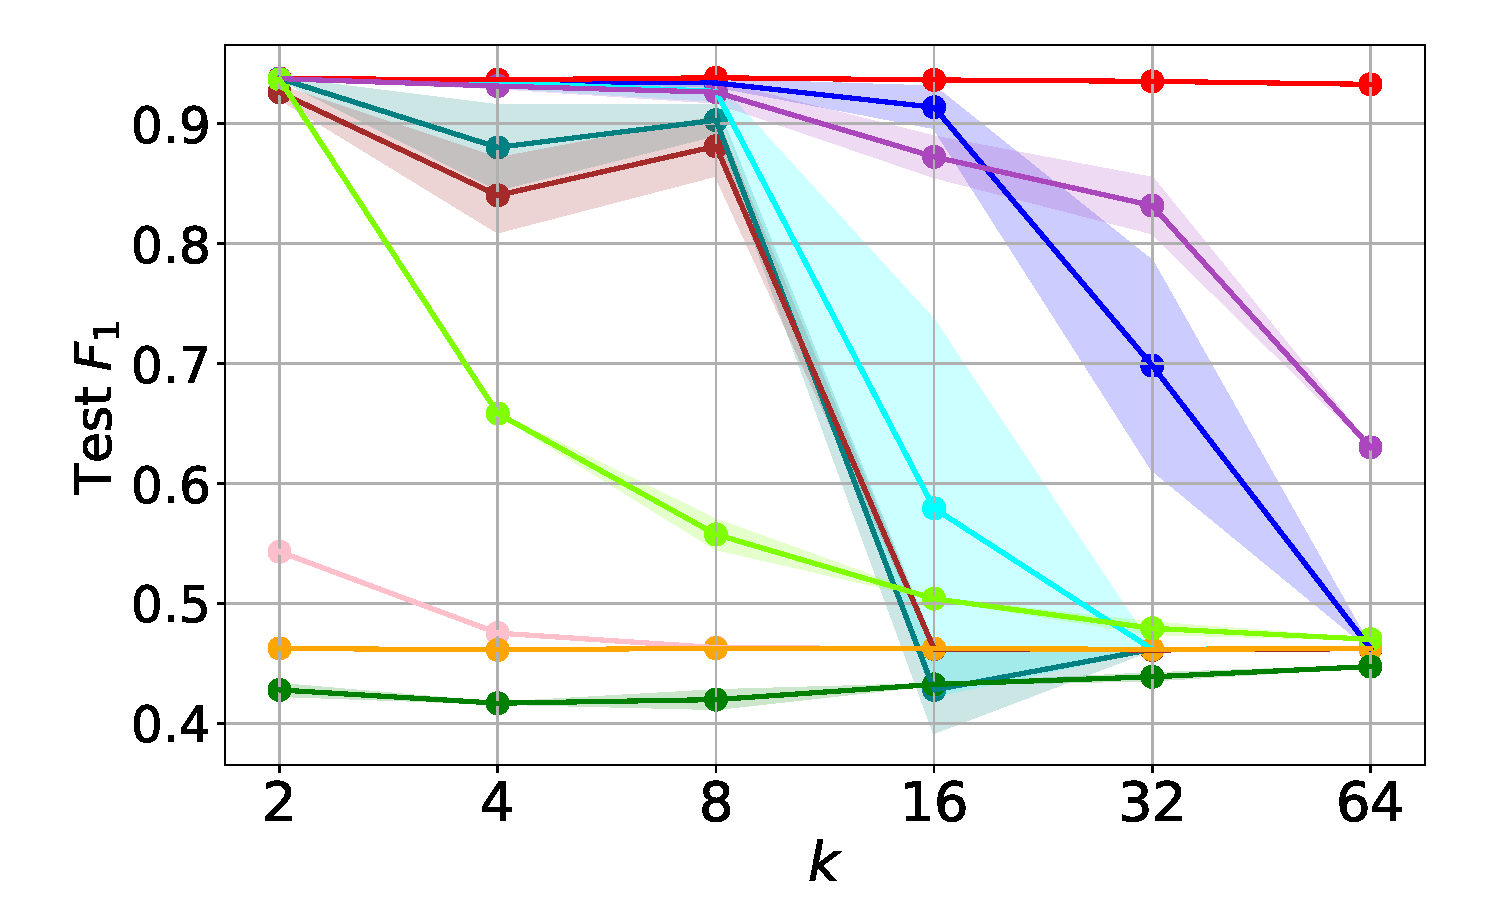
\includegraphics[width=0.35\linewidth]{figs/periodicity/sbm_sto/V2/(0.9, 0.01)(k, 1)All_test avg_f1.pdf}%
        \hspace{0.5cm}%
        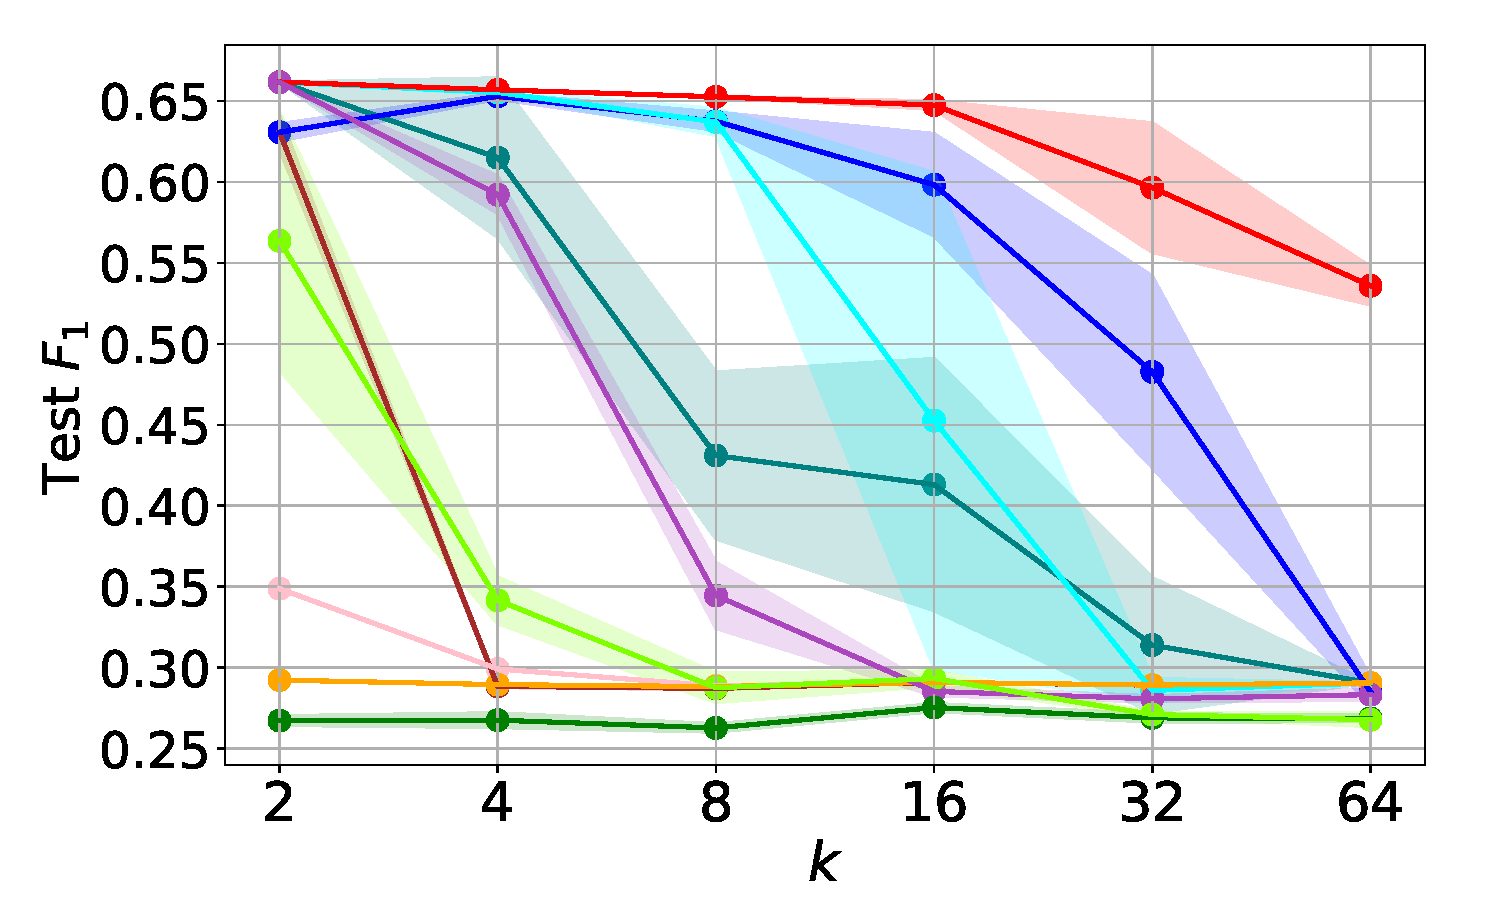
\includegraphics[width=0.35\linewidth]{figs/periodicity/sbm_sto/V2/(0.5, 0.01)(k, 1)All_test avg_f1.pdf}%
        %\hspace{1cm}%
        \raisebox{5mm}{
        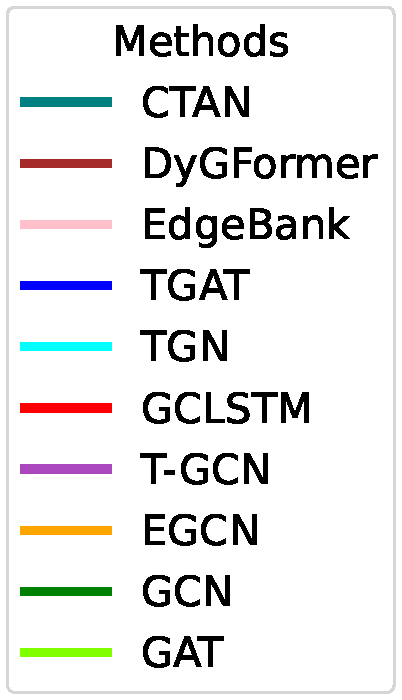
\includegraphics[width=0.08\linewidth]{figs/legends/CTDG DTDG all w edgebank wo persistence.pdf}}
    \caption{ Performance of TGL methods on the stochastic periodicity tasks~$\Psto{k,1}$ for different values of the intra-community edge probability: $p=0.9$ (left) and $p=0.5$ (right).
    }
    \label{fig:(K,1)_overall_sto}
\end{figure}

